%\chapter*{Appendix: The Kuhn-Tucker Theorem}
% \markboth{Appendix: The Kuhn-Tucker Theorem}{}

\begin{appendices}
\chapter{The Kuhn-Tucker Theorem} 
  
%\setcounter{equation}{0}
%\renewcommand\theequation{A.\arabic{equation}}

%\setcounter{figure}{0}
%\renewcommand{\thefigure}{A.\arabic{figure}}

The purpose of the Appendix is to offer the sketch of a rigorous proof of the Kuhn-Tucker Theorem, which is the most general theorem on first-order necessary conditions for maximization subject to non-negativity and inequality constraints. Notice the word `sketch': this is not a detailed proof, but each heuristic argument in the sketch can easily be converted into a rigorous one. This should suffice for most readers. I begin by recapitulating the statement of the theorem from Chapter 3:

\textit{Kuhn-Tucker Theorem:} Suppose $x$ is an $n$-dimensional vector, $c$ an $m$-dimensional vector, $F$ a function taking scalar values, $G$ a
function taking $m$-dimensional vector values. Define
\begin{equation*} \tag{3.4}
 L(x, \lambda) = F(x) + \lambda [c-G(x)]
\end{equation*}
where $\lambda$ is an $m$-dimensional row vector. Suppose $\bar{x}$ maximizes $F(x)$ subject to $G(x) \leq c$ and $x \geq 0$, and the constraint qualification holds, namely the submatrix of $G_x(\bar{x})$ formed by taking those rows $i$ for which $G^i(\bar{x}) = c$, has the maximum possible rank. Then there is a value of $\lambda$ such that
\begin{equation*} \tag{3.7}
L_x(\bar{x}, \lambda) \leq 0, \ \bar{x} \geq 0, \quad \mbox{with complementary slackness}
\end{equation*}
and
\begin{equation*} \tag{3.10}
L_\lambda(\bar{x}, \lambda) \geq 0,  \ \lambda \geq 0, \quad \mbox{with complementary slackness}
\end{equation*}

Before we begin the proof, we can simplify the notation. The non-negativity constraints can be expressed as $—x_j \leq 0 $ for $j = 1,2, \dots n$. Thus we can subsume them into the general inequality constraints, whose number $m$ is increased accordingly. We can also choose the labels on the component functions $G^i$ such that constraints $1, 2, \dots k$ are binding, and $k + 1, \dots m$ are slack, or
\begin{equation} \label{equaA.1}
G^i(\bar{x}) \left\{  \begin{array}{ll}
= c_i & \mbox{for} \  i=1,2,\dots k \\
< c_i & \mbox{for} \ i = k+1, \dots m 
\end{array}
\right.
\end{equation}

Since $\bar{x}$ is a maximizer (local or global) of $F(x)$ subject to $G(x) \leq c$, there is no neighboring $x$ such that 
\begin{equation} \label{equaA.2}
 G^i(x) \leq G^i(\bar{x}) = c_i  \quad \mbox{for} \ i=1,2,\dots k
\end{equation}
and
\begin{equation} \label{equaA.3}
F(x) > F(\bar{x})
\end{equation}
Note that we do not need any restrictions arising from the constraints $k+1, \dots m$; since the constraints hold as strict inequalities at $\bar{x}$, by continuity they will go on holding for $x$ sufficiently near $\bar{x}$.

Now write $x=\bar{x} +dx$ where $dx$ is infinitesimal. Then we want to replace (\ref{equaA.2}) and (\ref{equaA.3}) by the first-order Taylor approximations:
\begin{equation} \label{equaA.4}
 G_x^i(\bar{x}) dx \leq 0  \quad \mbox{for} \ i=1,2,\dots k
\end{equation}
and
\begin{equation} \label{equaA.5}
  F_x(\bar{x}) dx > 0
\end{equation}

This is valid provided the $k \times n$ matrix $G_x(\bar{x})$ formed by stacking the $k$ rows $G_x^i(\bar{x})$ has rank $k$. If it has a smaller rank, it has too large a null space, that is, too many vectors $dx$ yield zero when multiplied by this matrix. Then many more $dx$ satisfy the linear approximation (\ref{equaA.4}) than do $\bar{x} +dx$ satisfy the true constraints (\ref{equaA.2}). As a result, the first-order conditions can fail even though $\bar{x}$ is optimum.

I shall illustrate this using an example with two variables and two constraints. Suppose the objective function is 
\begin{equation*}
F(x_1, x_2) = x_1
\end{equation*}
and the constraints are
\begin{equation*}
 x_2 \geq x_1^3, \quad \mbox{or} \quad G^1(x_1, x_2) \equiv x_1^3 - x_2 \leq 0
\end{equation*}
\begin{equation*}
 x_2 \leq - x_1^3, \quad \mbox{or} \quad G^2(x_1, x_2) \equiv x_2 + x_1^3 \leq 0
\end{equation*}

\begin{figure}[!htb] %H为当前位置,!htb为忽略美学标准,htbp为浮动图形
\centering %图片居中
%\includegraphics[width=0.8\textwidth]{./Fig3.1.png} %插入图片,[]中设置图片大小,{}中是图片文件名
\begin{tikzpicture}[scale=1.0  ]
    % 绘制坐标轴
    \draw[->] (-5,0) -- (5,0) node[right] {$x_1$};
    \draw[->] (0,-4) -- (0,4) node[above] {$x_2$};
   % \draw[black] (0,0) node[below left] {$O$};

\fill[pattern=north west lines] plot[smooth,samples=100,domain=-4:0] (\x,{0.2*\x*\x}) -- plot[smooth,samples=100,domain=0:-4] (\x,{-0.2*\x*\x});
\draw[domain=-4:4,smooth,variable=\x, black] plot ({\x},{0.2* \x * \x  }) ;
\draw[domain=-4:4,smooth,variable=\x, black] plot ({\x},{-0.2* \x * \x  }) ;
 
\draw (4,3.2) node [above] {$G^1(x)=0$}; 
\draw (4,-3.2) node [below] {$G^2(x)=0$}; 
\end{tikzpicture}
\caption{Failure of the constraint qualification} %最终文档中希望显示的图片标题
\label{FigA.1} %用于文内引用的标签
\end{figure}
Figure \ref{FigA.1} shows the feasible set as the shaded area, and then it is clear that (0,0) solves the constrained maximization problem.

At this point both constraints bind $(k=2)$, and the vectors of derivatives of the constraints are
\begin{equation*}
G_x^1(0,0) = (0,-1) \quad \mbox{and} \quad G_x^2(0,0) = (0,1)
\end{equation*}
The rows are linearly dependent, and the rank of the matrix of derivatives is 1, which is <$k$. The linear approximation (\ref{equaA.4}) becomes
\begin{equation*}
 -dx_2 \leq 0 \quad \mbox{and} \quad dx_2 \leq 0, \quad \mbox{that is,} \quad dx_2=0
\end{equation*}
which is the whole horizontal axis. Points to the right of the origin are not in fact a linear approximation to the feasible set, but they appear as feasible deviations in the linear approximation to the functions.

Now we also see the sense of the remark made earlier in the context of linear programming (Example 7.1) that no constraint qualification was needed there. When the constraints are already linear, there is no need to find linear approximations to them, so the issue does not arise.
\begin{figure}[!htb] %H为当前位置,!htb为忽略美学标准,htbp为浮动图形
\centering %图片居中
%\includegraphics[width=0.8\textwidth]{./Fig3.1.png} %插入图片,[]中设置图片大小,{}中是图片文件名
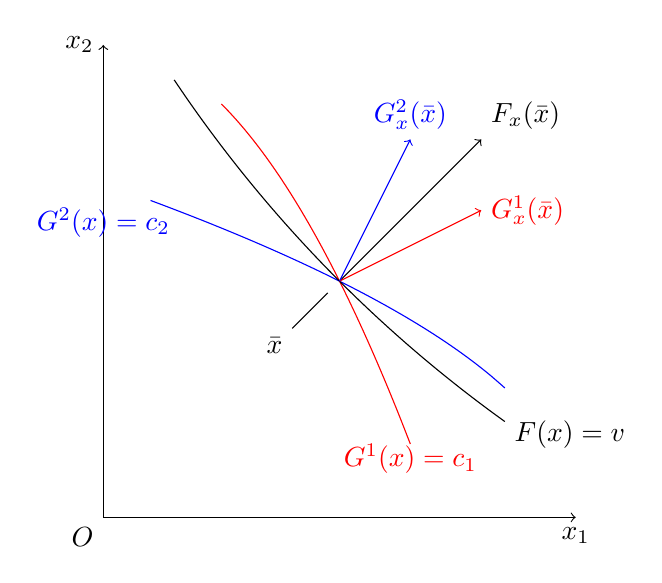
\begin{tikzpicture}[scale=3  ]
    % 绘制坐标轴
    \draw[->] (0,0) -- (2,0) node[below] {$x_1$};
    \draw[->] (0,0) -- (0,2) node[left] {$x_2$};
    \draw[black] (0,0) node[below left] {$O$};

\draw[domain=0.5:1.3,smooth,variable=\x, red] plot ({\x},{2 -  \x * \x  }) ;
\draw[domain=0.2:1.7,smooth,variable=\x, blue] plot ({\x},{ sqrt(2 -  \x)    }) ;
\draw[domain=0.3:1.7,smooth,variable=\x, black] plot ({\x},{ 5- sqrt(32 - (\x-5)*(\x-5) )  }) ;

\draw[->] (1,1) -- (1.6,1.6) node [above right] {$F_x(\bar{x})$} ;
\draw[->, red] (1,1) -- (1.6,1.3) node [right] {$G_x^1(\bar{x})$} ;
\draw[->, blue] (1,1) -- (1.3,1.6) node [above] {$G_x^2(\bar{x})$} ;


\draw[black] (0.95,0.95) -- (0.8,0.8) node[below left] {$\bar{x}$} ;
\draw[red] (1.3,0.35) node[below] {$G^1(x)=c_1$} ;
\draw[blue] (0,1.35) node[below] {$G^2(x)=c_2$} ;
\draw[black] (1.7,0.35) node[right] {$F(x)=v$} ;
\end{tikzpicture}
\caption{The Kuhn-Tucker Theorem} %最终文档中希望显示的图片标题
\label{FigA.2} %用于文内引用的标签
\end{figure}
Let us proceed with the assumption (the Constraint Qualification) that the rank of $G_x(\bar{x})$ equals $k$. Figure \ref{FigA.2} shows the situation. It is drawn so that all functions are increasing in $x$, but that is only to conform to the economic intuition; other configurations make no difference. The feasible region, and the upper contour set of $F(x)$ for its optimal value, are both shown by hatch-marks on their boundaries. The vector of derivatives of each of the functions is also shown; each is normal (perpendicular) to the contour curve of the corresponding function.

When $\bar{x}$ is optimum, the feasible region and the upper contour set of the objective function should not intersect. Assuming validity of the constraint qualification, their linear approximations defined by the deviations in (\ref{equaA.4}) and (\ref{equaA.5}) should not intersect either. For this to be true, the vector of derivatives $F_x(\bar{x})$ should lie in the cone formed by the vectors $G_x^i(\bar{x})$ of the derivatives of the constraint functions. This is more easily seen from the equivalent statement in the opposite direction (contrapositive) from the figure: if $F_x(\bar{x})$ were to lie outside this cone, the contour of $F$ through $\bar{x}$ would cut into the feasible region, so a neighboring feasible point with a higher value could be found, and $\bar{x}$ could not be optimal.

Points in a finite cone are non-negative linear combinations of the vectors that define the cone. Therefore there are non—negative numbers $\lambda_1, \lambda_2, \dots \lambda_k $ such that
\begin{equation} \label{equaA.6}
 F_x(\bar{x}) = \sum\limits_{i=1}^k \lambda_i G_x^i(\bar{x})
\end{equation}
It is harmless to extend the range of summation to $m$ by defining $\lambda_{k+1}, \dots, \lambda_m$ all equal to zero. The extended (\ref{equaA.6}) is just the condition $L_x( \bar{x}, \lambda) = 0$ to which (\ref{equa3.7}) reduces when there are no non-negativity constraints (remember they are subsumed into the inequality constraints and so do not have a separate role). The complementary slackness condition (\ref{equa3.10}) is fulfilled because of the way the $\lambda_i$ are defined for the slack constraints. This completes the sketch of the proof.

\end{appendices}






